%-----------------------------------------------------------------------------80
% SECTION TITLE
%-----------------------------------------------------------------------------80

\section{Utilidades}  

%-----------------------------------------------------------------------------80
% CONTENT
%-----------------------------------------------------------------------------80


\begin{frame}[fragile]{Utilidades}
\textbf{Argumentos por nombre}
 \begin{itemize}[<+(1)->]
    \item Un argumento por nombre o \emph{keyword} es un argumento ficticio, que "recuerda" una lista de argumentos de tal forma que permita identificarlos entre los argumentos de posición cuando se llama a un procedimiento.
        \begin{figure}
            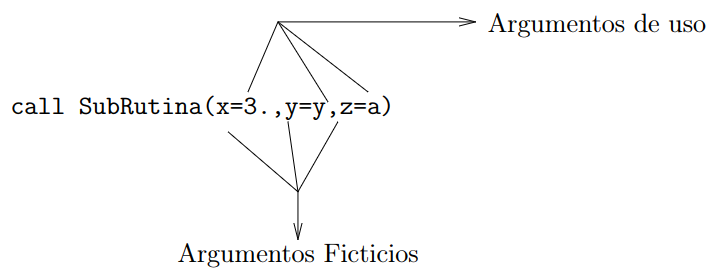
\includegraphics[width=0.5\textwidth]{./resources/keywords.png}
        \end{figure}
    \item Modifica el orden de los argumentos al llamar al procedimiento presenta las siguientes ventajas:
    \item [-] Permite que los argumentos reales se especifiquen en cualquier orden.
    \item [-] Ayudan a mejorar la legibilidad del programa.
    \item [-] Facilita agregar un argumento adicional sin la necesidad de modificar todas y cada una de las invocaciones en el código de llamada.
    \item Es posible definir los argumentos posicionales con los argumentos por nombre. 
    \item []
        \begin{minted}[linenos,autogobble]{fortran}
            CALL SubRutina (3.,y=y,z=a)
        \end{minted}
 \end{itemize}
\end{frame}

\begin{frame}[fragile]{Utilidades}
\textbf{Argumentos opcionales}
 \begin{itemize}[<+(1)->]
    \item 
 \end{itemize}
\end{frame}